\subsection{Bitmaps}
	The bitmap class consists of arrays, which contains bytedata of bitmap images, such as the intro image at the start of the game. 
	
	\begin{figure}[H]
		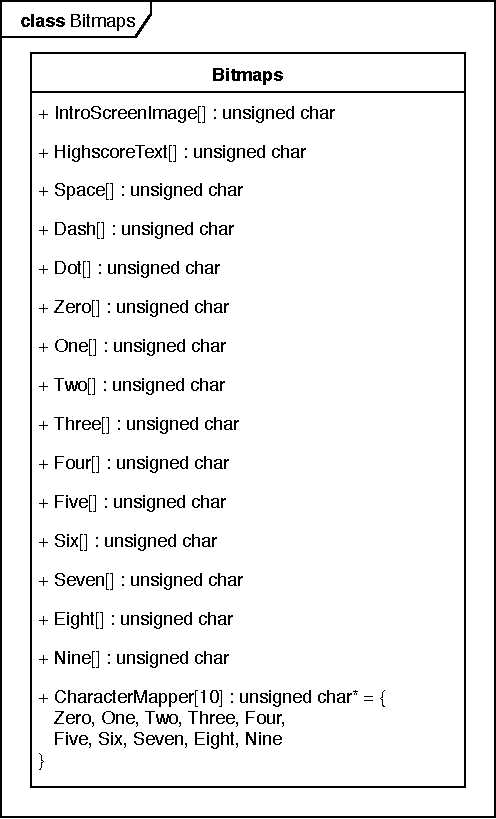
\includegraphics[scale=1.0]{BitmapsClassDiagram}
		\centering
		\caption{Class diagram for Bitmaps}
		\label{fig:classBitmap}
	\end{figure}
	
	The character arrays containing number data or other single character values have been named intuitively and they will not be described further. The CharacterMapper contains the number characters in an array to be able to access these using indices. IntroScreenImage and HighScoreText are bitmap images shown at the start and end of the game.
	
	All bitmaps have been created using LCD fontmaker \cite{FontMaker}. 